\section{Underlying Work}
\label{sec:underlying}

In this section we discuss the underlying work by \ca{sanchez2019can}. We talk about the methodology they use and the
results they achieved with their strategy.

The main focus of the underlying work is not to evaluate whether websites comply with the law, but rather to evaluate
the impact of the GDPR on the ability of a user to control their privacy online.

\subsection{Methodology}
\label{subsec:methodology}

The domain of their analysis are the Alexa top-1M websites. This is a web service by amazon which lists the websites with
the most traffic according to the Alexa Traffic Rank. From this list, they look at 2000 websites across different
categories from some of the top traffic websites.

The data collection was done manually. This means that \citeauthor{sanchez2019can} went through all the 2000 websites by
hand and noted features of the website. By doing this manually, you are less likely to miss any cookie notice or to
click something wrong. Cookie consent notices can differ tremendously from one website to another making it hard to
automate this task. On the other hand, collecting the data manually makes it harder to recreate the data they produced
and harder to look at different features afterwards because you do not want to manually go through the 2000 websites
again. Additionally, metrics like the waiting time until you decline the cookies or the waiting time until you reload
the page after declining cannot be captured by manual analysis. Manual analysis provides better error resistance but is
less flexible and practical than automated analysis. The data they collect are the cookies set before interacting with the
consent notice, the type of consent notice, the privacy policy and the cookies set after rejecting trackers if possible.
The different types of consent notices are:
\begin{enumerate}[a)]
    \item \emph{Anyway}: users are just informed that they are being tracked
    \item \emph{AutoAccept}: users are informed that by continuing to browse they accept tracking
    \item \emph{OnlyAccept}: there is only an accept button
    \item \emph{AcceptReject}: there is an accept and a reject button
    \item \emph{JustSettings}: there is a more complex settings dialog
\end{enumerate}
Cookie consent notices can be blocking and non-blocking meaning that you can access the website while the consent notice pops up for
non-blocking, and you cannot access the website until you have made a choice for blocking cookie consent notices. For
websites which link to third-party opt-out services(e.g. youronlinechoices), they used the service and observed the
cookie behavior.

The identification of tracking cookies was done through measuring the entropy of the value of a cookie with
\texttt{zxcvbn} \cite{wheeler2016zxcvbn}. If the entropy is high enough to distinguish you from 1 Billion people, they
consider it a tracking cookie. This is a rather new approach to the problem of identifying tracking cookies.
On one hand you can detect cookies which with other methods could have been missed, but on the other hand you can get false positives
where the cookie was not a tracker, but it was still classified as one. The latter is not a problem since the
GDPR specifies that cookies which carry information that in theory could identify you still require consent even if they
are not used as tracking cookies.
A more common approach is to make use of lists of known third-party trackers. This approach cannot reliably identify
first-party trackers and can miss some unknown third-parties. \citeauthor{sanchez2019can} use third-party tracker lists
to classify their found trackers.

The GDPR requires privacy policies to be readable. Often, the privacy settings (e.g. cookie control) are only presented
in the privacy policy section of a website. \citeauthor{sanchez2019can} evaluate the difficulty of privacy policies with
two metrics, the \emph{Flesch Reading Ease Score} (FRES)~\cite{flesch1948new} and the \emph{Flesch-Kincaid Reading
Level} (FKRL)~\cite{kincaid1975derivation}. Both metrics evaluate the difficulty of texts through number of syllables
per word and sentence length. A score of about 50 could be seen as an average reading difficulty and FRES has an upper
bound of 121.22 (greater equals easier text) and no theoretical lower bound. FKRL has a lower bound of -1.3 and no
theoretical upper bound. \ca{jensen2004privacy} also use these metrics making it easier to compare their results to the
results of this paper.

\subsection{Evaluation}

In this subsection we highlight some of the main results of the underlying work.

\subsubsection{Tracking}

\begin{figure}
    \centering
    \begin{subfigure}[b]{.5\textwidth}
        \centering
        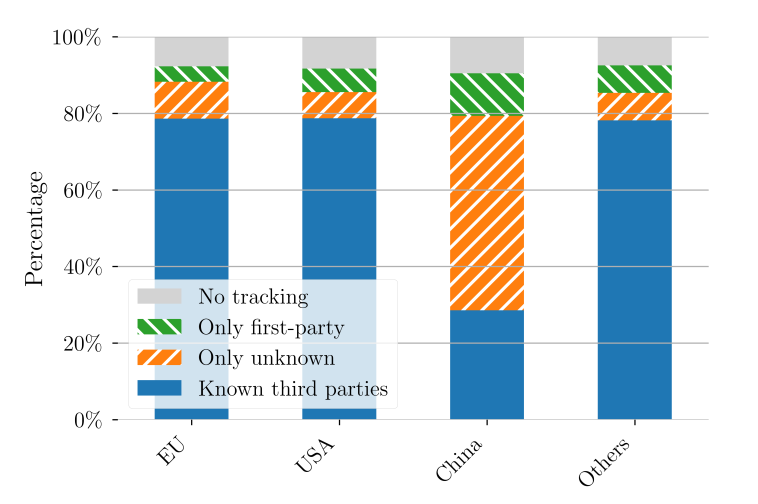
\includegraphics[width=\textwidth, scale=0.32]{figures/tracking_kind_trans.png}
        \caption{Kind of tracking observed.\\Figure by \citeauthor{sanchez2019can}~\cite[Fig.~1]{sanchez2019can}.}
        \label{fig:tracking_kind}
    \end{subfigure}
    \begin{subfigure}[b]{.5\textwidth}
        \centering
        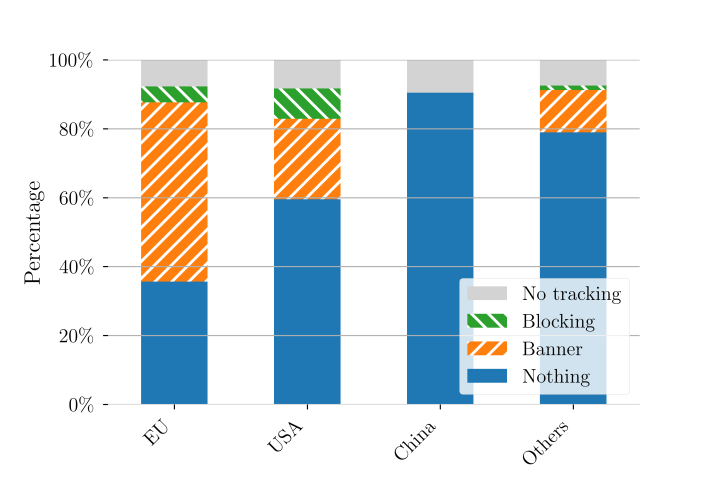
\includegraphics[width=\textwidth, scale=0.35]{figures/cookie_notice_size_trans.png}
        \caption{The size of the cookie notice.\\Figure by \citeauthor{sanchez2019can}~\cite[Fig.~2a]{sanchez2019can}.}
        \label{fig:notice_size}
    \end{subfigure}
    \begin{subfigure}[b]{.5\textwidth}
        \centering
        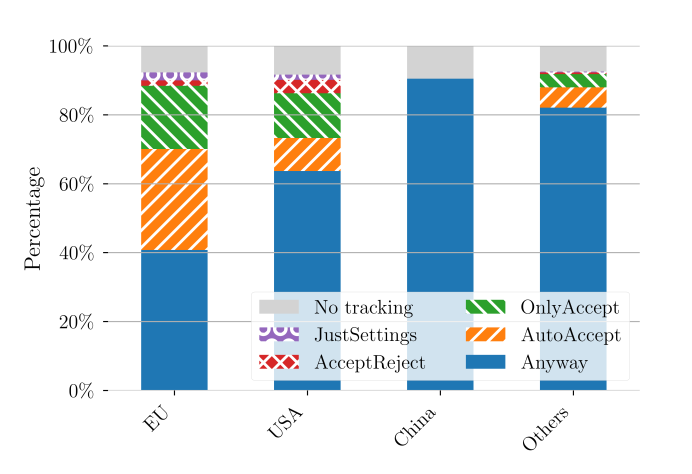
\includegraphics[width=\textwidth, scale=0.35]{figures/cookie_notice_type_trans.png}
        \caption{Type of cookie notice.\\Figure by \citeauthor{sanchez2019can}~\cite[Fig.~2b]{sanchez2019can}.}
        \label{fig:notice_type}
    \end{subfigure}
    \caption{Statistics about cookie tracking and consent notices}
    \label{fig:cookie_stats}
\end{figure}

\autoref{fig:cookie_stats} shows the evaluations of the underlying work that we want to focus on.

\autoref{fig:tracking_kind} illustrates the kind of tracking on the visited websites. We can observe that about 92\% of
the websites perform some kind of tracking. This tracking is done before any consent is given and even after rejecting
tracking cookies (opt-out). Many websites make use of third-party tracking and only a few use first-party tracking. We
can also criticize this figure because we cannot see how many websites that use known third-party tracking also use
first-party tracking because all websites that use third-party tracking are thrown into one category.

\autoref{fig:notice_size} shows the size of the cookie notice differentiating between cookie consent notices which block
you from accessing a website until you have made a choice on cookies, banners which do not block you from browsing the
website and no cookie consent notice (splitting websites that do perform tracking and websites that do not and have no
cookie consent notice). The GDPR specifies that consent must be explicit before any kind of tracking is performed
(opt-in instead of opt-out) meaning that no cookie consent notice despite tracking is illegal.
We can see in \autoref{fig:notice_size} that around 57\% of EU websites and 32\% of US
websites have some form of cookie notice showing that the GDPR has an impact on the amount of cookie notices.
Chinese websites do not display any cookie consent notice.

\autoref{fig:notice_type} shows the type of cookie consent notice as discussed in \autoref{subsec:methodology}.
We can observe that most websites do not have an easy way to opt-out. The best practices like \emph{AcceptReject} and
\emph{JustSettings} are almost not present in any cookie consent notice. If a website has a cookie consent notice, it
most likely just informs the user that cookies are being used.

This shows that the GDPR had the impact of getting more
cookie consent notices onto websites, but these are often useless as they are not conform wit the GDPR and users are
tracked even if they reject anyway.

A critique point here is that the evaluation of \ca{sanchez2019can} is lacking a proper comparison of the time before
the GDPR and the time after. They only show their results in a post GDPR world leading to some statements being out of
context (e.g. There are no numbers on how many cookie consent notices there were in the EU before the GDPR).

\subsubsection{Privacy Policies}

\TODO{privacy policies}

